\documentclass[11pt,letterpaper,fleqn]{article}
\usepackage{rotating}
\usepackage{graphicx}
\usepackage{amsfonts,amsmath}
\usepackage{subfigure} % need for subfigures
\usepackage{wrapfig}
\usepackage[margin=1in]{geometry}
\usepackage{cite}
\usepackage{amssymb}
\usepackage[final]{pdfpages}
\usepackage{hyperref,enumitem}
\hypersetup{
colorlinks, citecolor=blue, filecolor=black, linkcolor=blue, urlcolor=blue}
\usepackage{booktabs}
\usepackage{multirow}
\usepackage{siunitx}
\sisetup{group-separator = {,}}
\usepackage{titlesec}
\titlespacing\section{0pt}{6pt plus 4pt minus 2pt}{0pt plus 0pt minus 0pt}
\titlespacing\subsection{0pt}{6pt plus 4pt minus 2pt}{0pt plus 0pt minus 0pt}
\titlespacing\subsubsection{0pt}{6pt plus 4pt minus 2pt}{0pt plus 0pt minus 0pt}
\usepackage{titling} % Allows custom title configuration
\usepackage{fancyhdr} % Needed to define custom headers/footers
\usepackage{lastpage} % Used to determine the number of pages in the document
\usepackage[english]{babel}
\usepackage{blindtext}
%\usepackage{draftwatermark}
%\SetWatermarkText{Draft v0.0}

% Add you own definitions here (file report-defs.sty).
\usepackage{report-defs}
%\setlength{\headheight}{130pt}% ...at least 51.60004pt
\usepackage{tikzpagenodes}

%-------------------------------------------------------------------------------
%   TITLE SECTION
%-------------------------------------------------------------------------------

\date{} % blank out date from fancyhdr

\pretitle{
\vspace{-50pt}
\begin{flushleft} \fontsize{15}{15} \usefont{OT1}{phv}{b}{n} \selectfont} % Horizontal rule before the title
\title{\large Summary of Blueprint Workshop: \\
\vspace{1pt}
%\color{red}
\LARGE \textit{Analysis Systems R\&D on Scalable Platforms} \\
\color{black} \normalsize
\vspace{10pt}
June 21--22, 2019 \\
New York University \\
Meeting URL: \href{https://indico.cern.ch/event/820946/}{https://indico.cern.ch/event/820946/}
} % Your article title
\posttitle{\par\end{flushleft}\vskip 0.5em} % Whitespace under the title
\preauthor
{
  \begin{flushleft}
    \vspace{-13pt}
    {\normalfont Workshop Organizers:} \\
    \vspace{3pt}
    \large \lineskip 0.5em \usefont{OT1}{phv}{b}{sl} \color{black}} % Author font configuration
    \author{Kyle Cranmer {\normalfont(New York University)}
      \and  Rob Gardner {\normalfont(University of Chicago)}
      \and  Mark Neubauer {\normalfont(University of Illinois at Urbana-Champaign)}
      }
      \postauthor{\par
      \vspace{10pt}
      {\normalfont Summary prepared by:} \\
      \vspace{3pt}
      Mark Neubauer {\normalfont(University of Illinois at Urbana-Champaign)}

\end{flushleft} \vspace{-10pt} \HorRule} % Horizontal rule after the title

\renewcommand{\and}{\\}

%-------------------------------------------------------------------------------

\begin{document}
\maketitle % Print the title
\normalfont

\thispagestyle{firststyle}

\vspace{-250pt}
\hspace{360pt}

\includegraphics[height=30mm]{../../../figures/iris-hep-bluprint-logo.png}

\vspace{120pt}
\section*{Major Goals}
\vspace{3pt}
\begin{itemize}
  \item Review the status of the Analysis Systems (AS) milestones and deliverables from a perspective of needs for a collaborative development and testing platform.
  \item Develop the Scalable Systems Laboratory (SSL) scope, architecture and plans, using AS R\&D activities as concrete examples.
  \item Develop requirements on SSL to support the AS area, particularly the prototyping, benchmarking and scaling of AS deliverables toward production deployment.
  \item Increase the visibility of SSL and AS R\&D beyond IRIS-HEP to facilitate partnerships with organizations that could potentially provide software and computing resources toward these objectives.
  \item Get informed on latest developments in open source technologies and methods relevant for SSL and AS.
\end{itemize}

\section*{Key Outcomes}
\vspace{3pt}
\begin{itemize}
  \item Communication of the AS area plans and a preliminary set of requirements to SSL team.
  \item Kubernetes identified as a planned {\it common denominator} technology for the SSL, increasing innovation capability through flexible infrastructure.  This idea spawned plans for a multi-site SSL {\it substrate} project that will federate SSL contributions from multiple resource providers (institutes and public cloud), offering the AS area a flexible platform for service deployment at scales needed to test the viability of system designs.
  \item Productive engagement of the AS/SSL team with representatives from NCSA, SDSC, NYU Research Computing, industry \& cloud providers (Google, Redhat), generating action items and informing Year 2 planning of IRIS-HEP.
  \item A concrete vision for an SSL that serves not only as an innovation space for AS developers, but as a testbed to prototype next generation infrastructure patterns for future HEP computing environments.
\end{itemize}

%-------------------------------------------------------------------------------

\newpage
\pagestyle{reststyle}

\section{Overview}
\vspace{0.2cm}
Together with the OSG-LHC, the Scalable Systems Laboratory (SSL) is designed to assist integration and delivery of IRIS-HEP R\&D products targeted for the distributed and scientific production infrastructure of the experiments. The aim of this workshop is to further develop the IRIS-HEP SSL concept using specific examples from the Analysis Systems (AS) R\&D area, including low-latency, query-based data analyis systems and modular, reusable cyberinfrastructure for parameter fitting, physics inference and results dissemination. Registered attendees included those from IRIS-HEP (primarily from the SSL and AS focus areas), US ATLAS/CMS operations programs, DOE national and CERN laboratories, supercomputing centers (SDSC, NCSA), university research IT organizations, and industry (RedHat, Google).

The venue for the Blueprint workshop was the Physics Department at New York University (NYU) and was hosted by Kyle Cranmer who is a member of the NYU faculty an the IRIS-HEP Analysis Systems Coordinator. The workshop benefited from its proximity to the IRIS-HEP \href{https://indico.cern.ch/event/822074/}{Analysis Systems Topic Workshop} which immediately proceeded it and the \href{https://indico.cern.ch/event/765245/}{ATLAS Software and Computing Week} which directly followed -- all three events were hosted by NYU in a span of two weeks at the end of June 2019.

\section{Attendees}
\vspace{0.2cm}
There were 26 \href{https://indico.cern.ch/event/820946/registrations/participants}{registered participants} for workshop, with all but a few attending in person. The US ATLAS and US CMS computing operations and physics support managers were solicited in advance to send representatives from program areas with related interests, such as analysis framework developers and infrastructure providers.

The workshop attendees were:
Andrew Chien (Chicago),
Andrew Melo (Vanderbilt),
Aravindh Puthiyaparambil (Red Hat),
Benjamin Galewsky (Illinois/NCSA),
Dan S. Katz (Illinois/NCSA),
David Ackerman (NYU),
Edgar Fajardo (SDSC),
Eric Borenstein (NYU),
Gordon Watts (Washington),
Ianna Osborne (Fermilab),
Jim Pivarski (Princeton),
Kyle Cranmer (NYU),
Lincoln Bryant (Chicago),
Lindsey Gray (Fermilab),
Mark Neubauer (Illinois),
Mason Proffitt (Washington),
Matthew Feickert (SMU),
Nils Krumnack (Iowa State),
Ricardo Brito Da Rocha (CERN),
Rob Gardner (Chicago),
Sanjay Arora (Red Hat),
Stephen Fang (Google),
Stratos Efstathiadis (NYU),
Tatiana Polunina (NYU),
Tim Boerner (Illinois/NCSA),
Wei Yang (SLAC).

\section{Goals}
\label{sec:Goals}
\vspace{0.2cm}
As an IRIS-HEP Blueprint activtiy, the workshop was broadly designed to inform the development and evolution of the Institute’s strategic vision by bringing together team members, key stakeholders and domain experts from disciplines of importance to the Institute's mission. Specific to the workshop theme of \textit{Analysis System R\&D on Scalable Platforms}, the organizers set forth several goals in advance of the workshop. The key goals of the workshop were to:

\begin{itemize}
  \item Review the status of Analysis Systems (AS) milestones and deliverables to identify the needs for collaborative development and testing platforms in the AS R\&D area.
  \item Further develop the Scalable Systems Laboratory (SSL) concept, scope, architecture and plans, using R\&D activities from the AS area as specific examples.
  \item Develop requirements on SSL to support the AS area, particularly the prototyping, benchmarking and scaling of AS deliverables toward integrating within the LHC experiments.
  \item Increase the visibility of SSL and AS R\&D area beyond IRIS-HEP to facilitate partnerships with organizations that could potentially provide software and computing resources for SSL.
  \item Extend knoweledge within the Institute of current developments in technologies and methods relavent for SSL and the AS R\&D area from participation by scientists in other domains and industry partners.
\end{itemize}

Significant progress was made towards each of these goals over the 1.5 day workshop. The Blueprint meeting itself satisfied an AS area milestone, namely Milestone {\bf G2.5} "Blueprint workshop coordinating resource needs for evaluating analysis systems coordinated by SSL with participation of operations program" under WBS 2.3 of the IRIS-HEP \textit{Project Execution Plan}.

\section{Activites}
\vspace{0.2cm}
The meeting was structured as a series of informal presentations and discussion blocks to allow sufficient time for in-depth discussions.  In advance of the meeting, we identified a number of questions and topics to guide the discussions, including:

\begin{itemize}
  \item Collection of analysis use cases, each with a reference implementation.  What patterns and infrastructure are needed?
  \item Translation of analysis examples into infrastructure environments providing feedback for development iterations.
  \item Development of initial specifications for developer-facing interfaces for analysis system components.
  \item Benchmarking of existing analysis components and integrating the benchmarking into SSL.
  \item Identifying needs for development of accelerator-based fitting \& statistical tools (and other relevant components).
  \item Integrating prototypes of AS components into SSL, followed by benchmarking \& assessment.
\end{itemize}

\subsection{Presentations and Discussion}
\vspace{0.2cm}
There were 9 formal presentations delivered to trigger discussion on the main themes and objectives of the workshop:

\vspace{0.2cm}

\noindent~~~$\bullet$~\href{https://indico.cern.ch/event/820946/contributions/3461588/attachments/1866577/3069573/IRIS-HEP_BluePrint_AS_SSL.pdf}{\textbf{\textit{IRIS-HEP Blueprint Concepts and Process}}} (Mark Neubauer / Illinois)

\noindent~~~$\bullet$~\href{https://indico.cern.ch/event/820946/contributions/3461590/attachments/1866979/3070394/2019.06.21_SSL_Overview_Rob.pdf}{\textbf{\textit{Scalable Systems Laboratory: Challenges, \& Opportunities}}} (Rob Gardner / Chicago)

\noindent~~~$\bullet$~\href{https://indico.cern.ch/event/820946/contributions/3461589/attachments/1867063/3070546/AS-SSL-Blueprint.pdf}{\textbf{\textit{Analysis Systems Perspectives \& Goals}}} (Kyle Cranmer / NYU)

\noindent~~~$\bullet$~\href{https://indico.cern.ch/event/820946/contributions/3461592/attachments/1866998/3119402/2019.06.21_SSL_Patterns__Deployments_Lincoln.pdf}{\textbf{\textit{SSL Hybrid Models, Developer Support \& Deployments}}} (Lincoln Bryant / Chicago)

\noindent~~~$\bullet$~\href{https://indico.cern.ch/event/820946/contributions/3461593/attachments/1867157/3070768/go}{\textbf{\textit{Use of the Google Cloud Platform in High-Energy Physics}}} (Lukas Heinrich / CERN)

\noindent~~~$\bullet$~\href{https://indico.cern.ch/event/820946/contributions/3461594/attachments/1867161/3070777/OpenShift_4.pdf}{\textbf{\textit{RedHat OpenShift}}} (Sanjay Arora / RedHat)

\noindent~~~$\bullet$~\href{https://indico.cern.ch/event/820946/contributions/3461593/attachments/1867157/3070794/go}{\textbf{\textit{Google Perspective}}} (Stephan Fang / Google)

\noindent~~~$\bullet$~\href{https://indico.cern.ch/event/820946/contributions/3461596/attachments/1867159/3070772/go}{\textbf{\textit{Research Computing Technology at NYU}}} (David Ackerman / NYU)

\noindent~~~$\bullet$~\href{https://indico.cern.ch/event/820946/contributions/3464565/attachments/1867166/3070786/IRIS-HEP-Accelerated-Scalability-6-21-2019-v2.pdf}{\textbf{\textit{Accelerated Systems \& Optimization}}} (Andrew Chien / Chicago) \\

\vspace{-0.2cm}
During the afternoon session, Ben Galewsky (Illinois/NCSA) presented an architectural diagram, some ideas about implemntation, and current status of ServiceX, which is aimed at accelerated delivery of data (often transformed) for analysis as part of the Intelligent Data Delivery Service (iDDS) (see Figure~\ref{fig:galewsky_servicex}). The iDDS was conceived in the
\begin{wrapfigure}[21]{R}{0.47\textwidth}
  \centering
  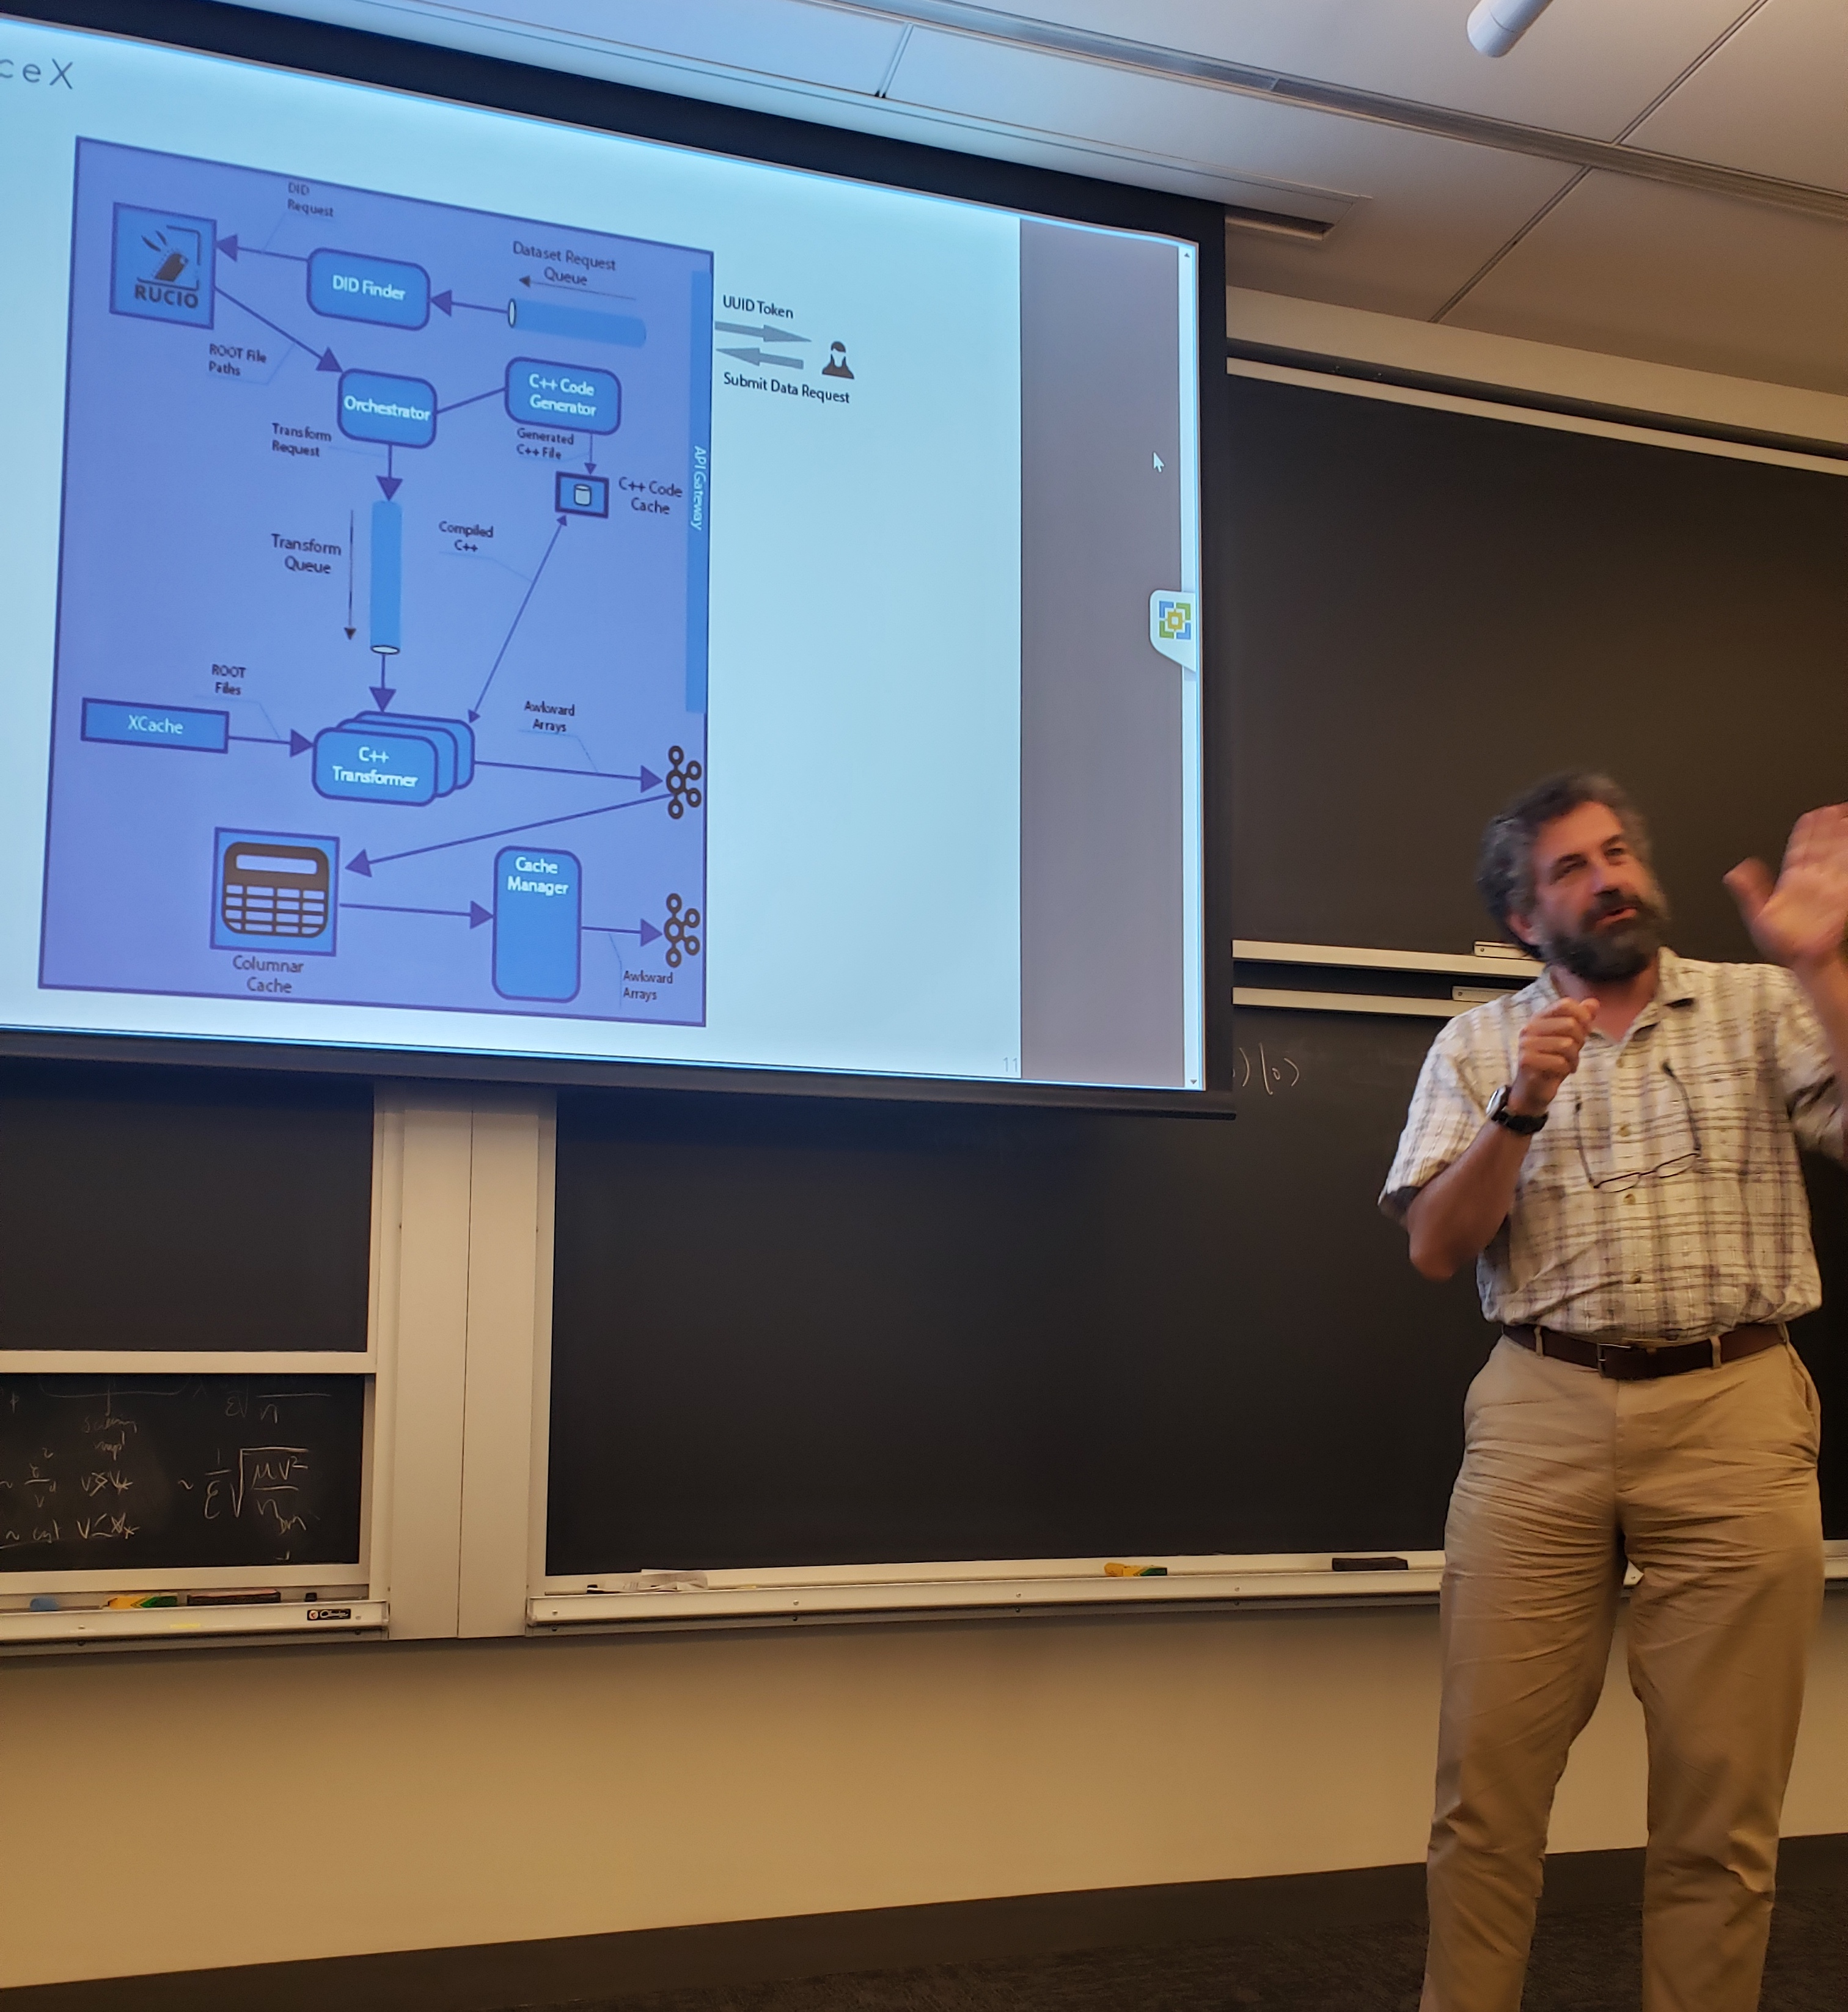
\includegraphics[width=0.9\linewidth]{figures/galewsky_servicex.jpg}
  \vspace{-0.3cm}
  \caption{Ben Galewsky (Illinois) presents on an accelerated delivery and transformation service for analysis data (ServiceX) as part of the Intelligent Data Delivery Service (iDDS).}
  \label{fig:galewsky_servicex}
\end{wrapfigure}
conceptualization phase of IRIS-HEP and developed as an early R\&D target in the Data Organization, Management and Access area.

In the afternoon discussion block, participants identified potential contributing partners to SSL along with specific resource targets, where applicable. Representative(s) from potential partner sites were present in some cases, for example Tim Boerner at the National Center for Supercomputing Applications and Edgar Fajardo at the San Diego Supercomputing Center. The group engaged in something of a round table those in attendence to affirm their interests in working with SSL, discuss their capabilities and develop plans for making their resources available to IRIS-HEP.

\subsubsection{The Blueprint Process}
\vspace{0.2cm}
Mark Neubauer (Illinois) presented \href{https://indico.cern.ch/event/820946/contributions/3461588/attachments/1866577/3069573/IRIS-HEP_BluePrint_AS_SSL.pdf}{\it IRIS-HEP Blueprint Concepts and Process} which provided a broad overview of the goals of particles and the LHC experiments, including the technical and computing challenges they will face in the HL-LHC era and the role that software will play in addressing those challenges. A brief history of the Blueprint activity in development of the Institute was presented, along with a description of process by which it informs the development and evolution of the strategic vision and the roll it plays in IRIS-HEP as an intellectual hub for HEP software \& computing (see Figure~\ref{fig:overview}). This was followed by a discussion of the major major goals for the AS/SSL Blueprint Workshop. \begin{wrapfigure}[19]{R}{0.47\textwidth}
  \centering
  \vspace{-0.4cm}
  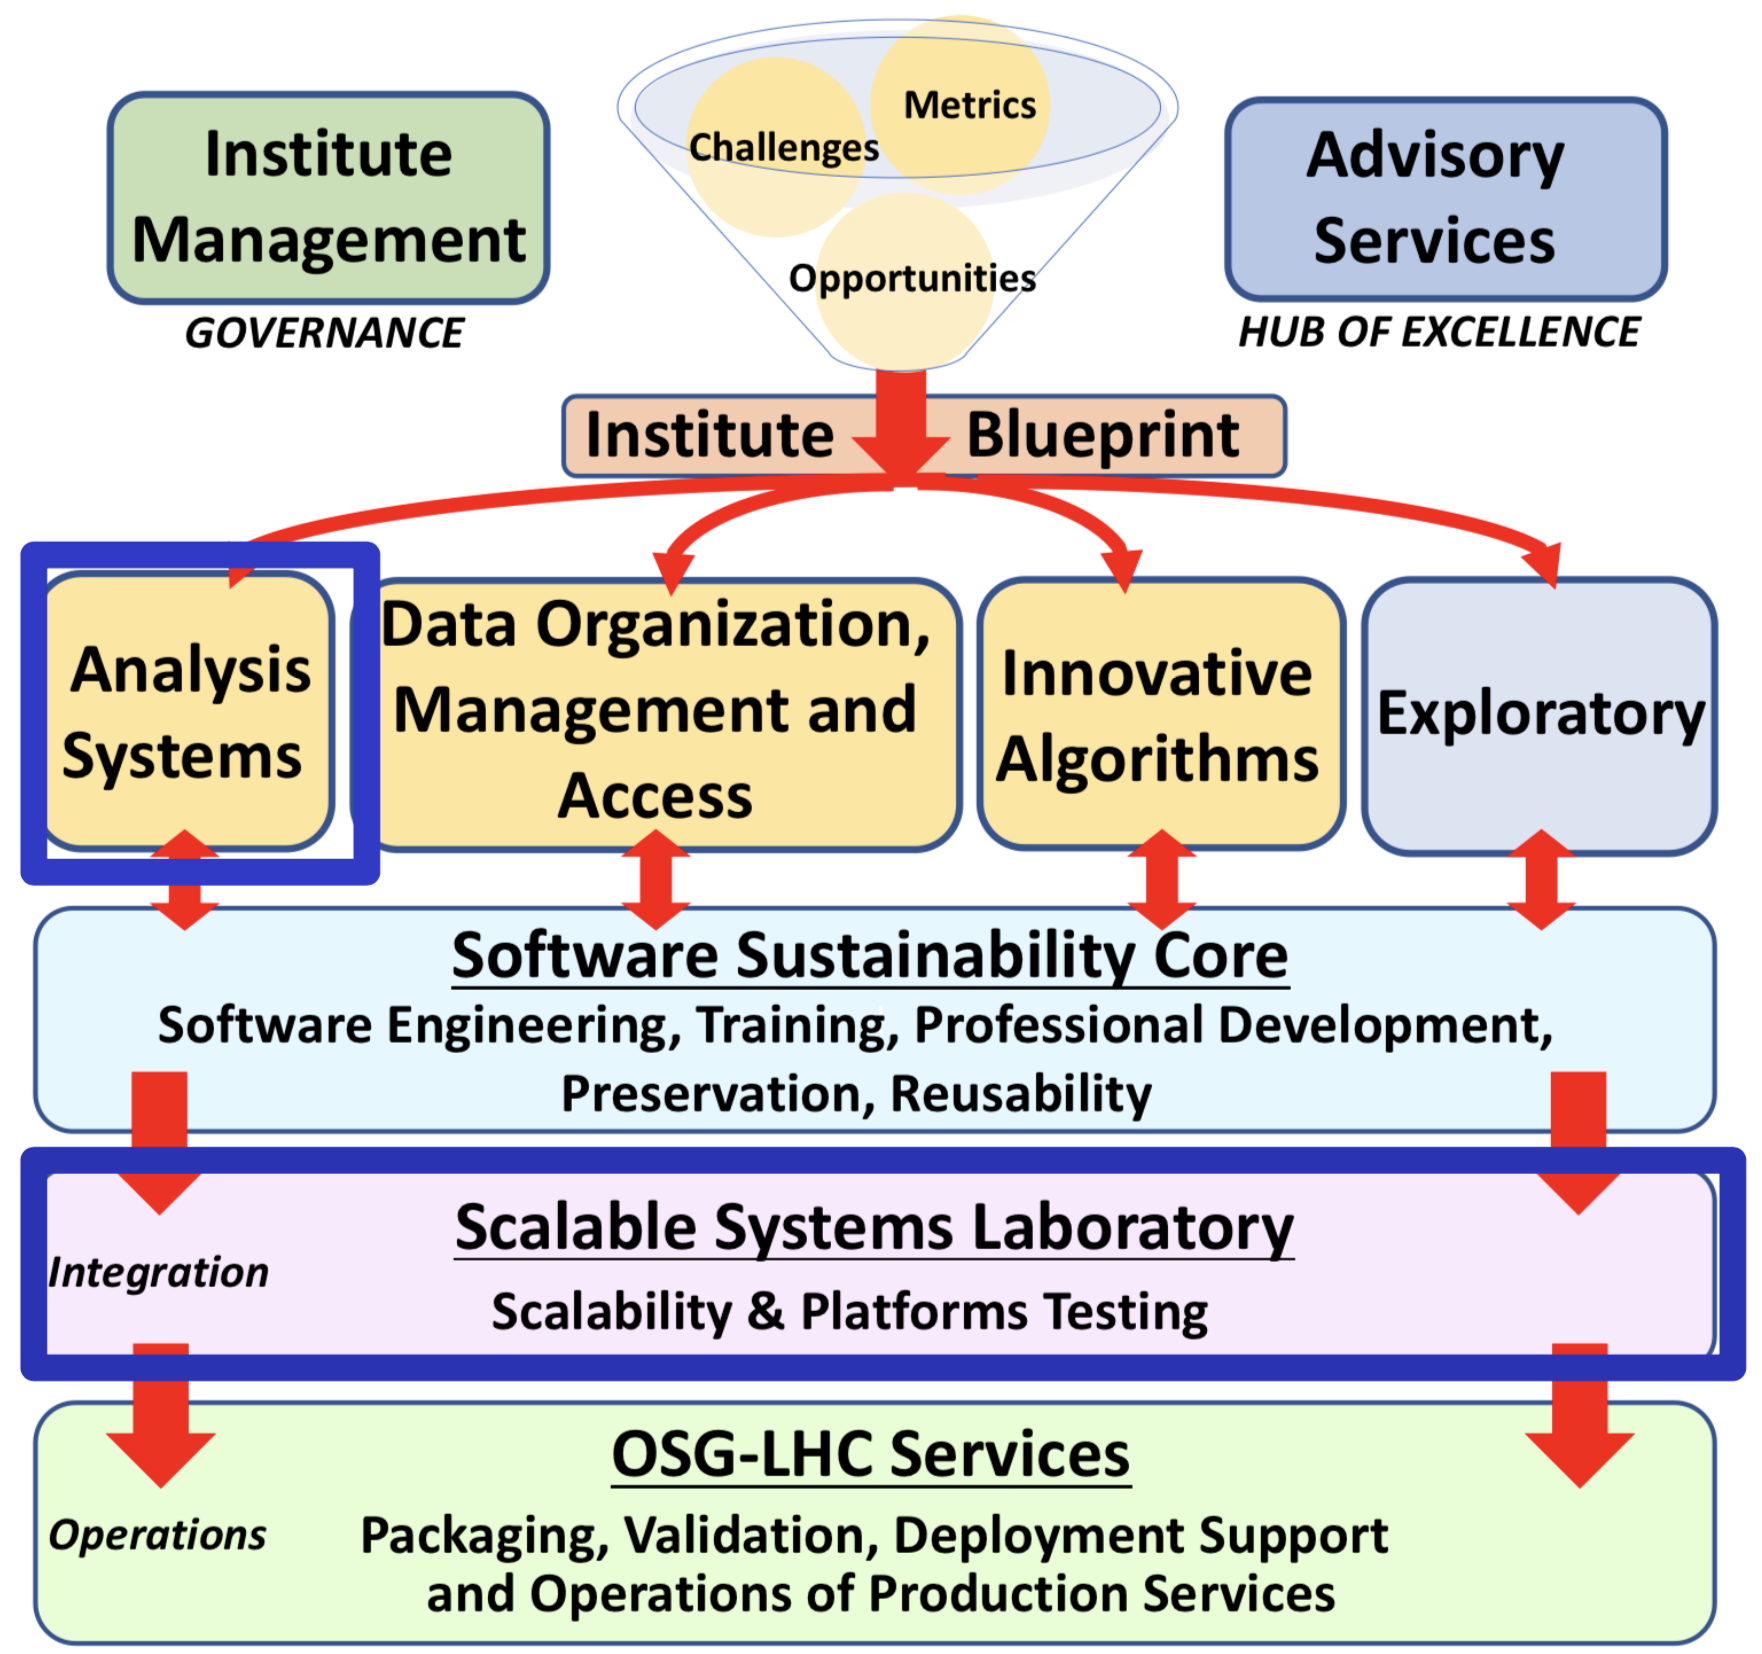
\includegraphics[width=0.99\linewidth]{figures/AS_SSL_IRIS-HEP.png}
  \vspace{-0.7cm}
  \caption{Overview of the IRIS-HEP areas, with AS and SSL as the focus of this Blueprint Workshop indicated with blue boxes.}
  \label{fig:overview}
\end{wrapfigure}

Feedback was reeived that this overview was particularly helpful to workshop participants new to computing in HEP and unaware of the scale of the HL-LHC computing challenges, helping put the data and processing challenges in context.

\subsubsection{The SSL Concept}
\vspace{0.2cm}
Robert Gardner (Chicago) presented \href{https://indico.cern.ch/event/820946/contributions/3461590/attachments/1866979/3070394/2019.06.21_SSL_Overview_Rob.pdf}{\textit Scalable Systems Laboratory: Challenges, \& Opportunities} in which the concept was discussed and the initial program of work was described (Figure~\ref{fig:rwg_ssl}). Given that
\begin{wrapfigure}[20]{L}{0.48\textwidth}
  \vspace{-0.4cm}
  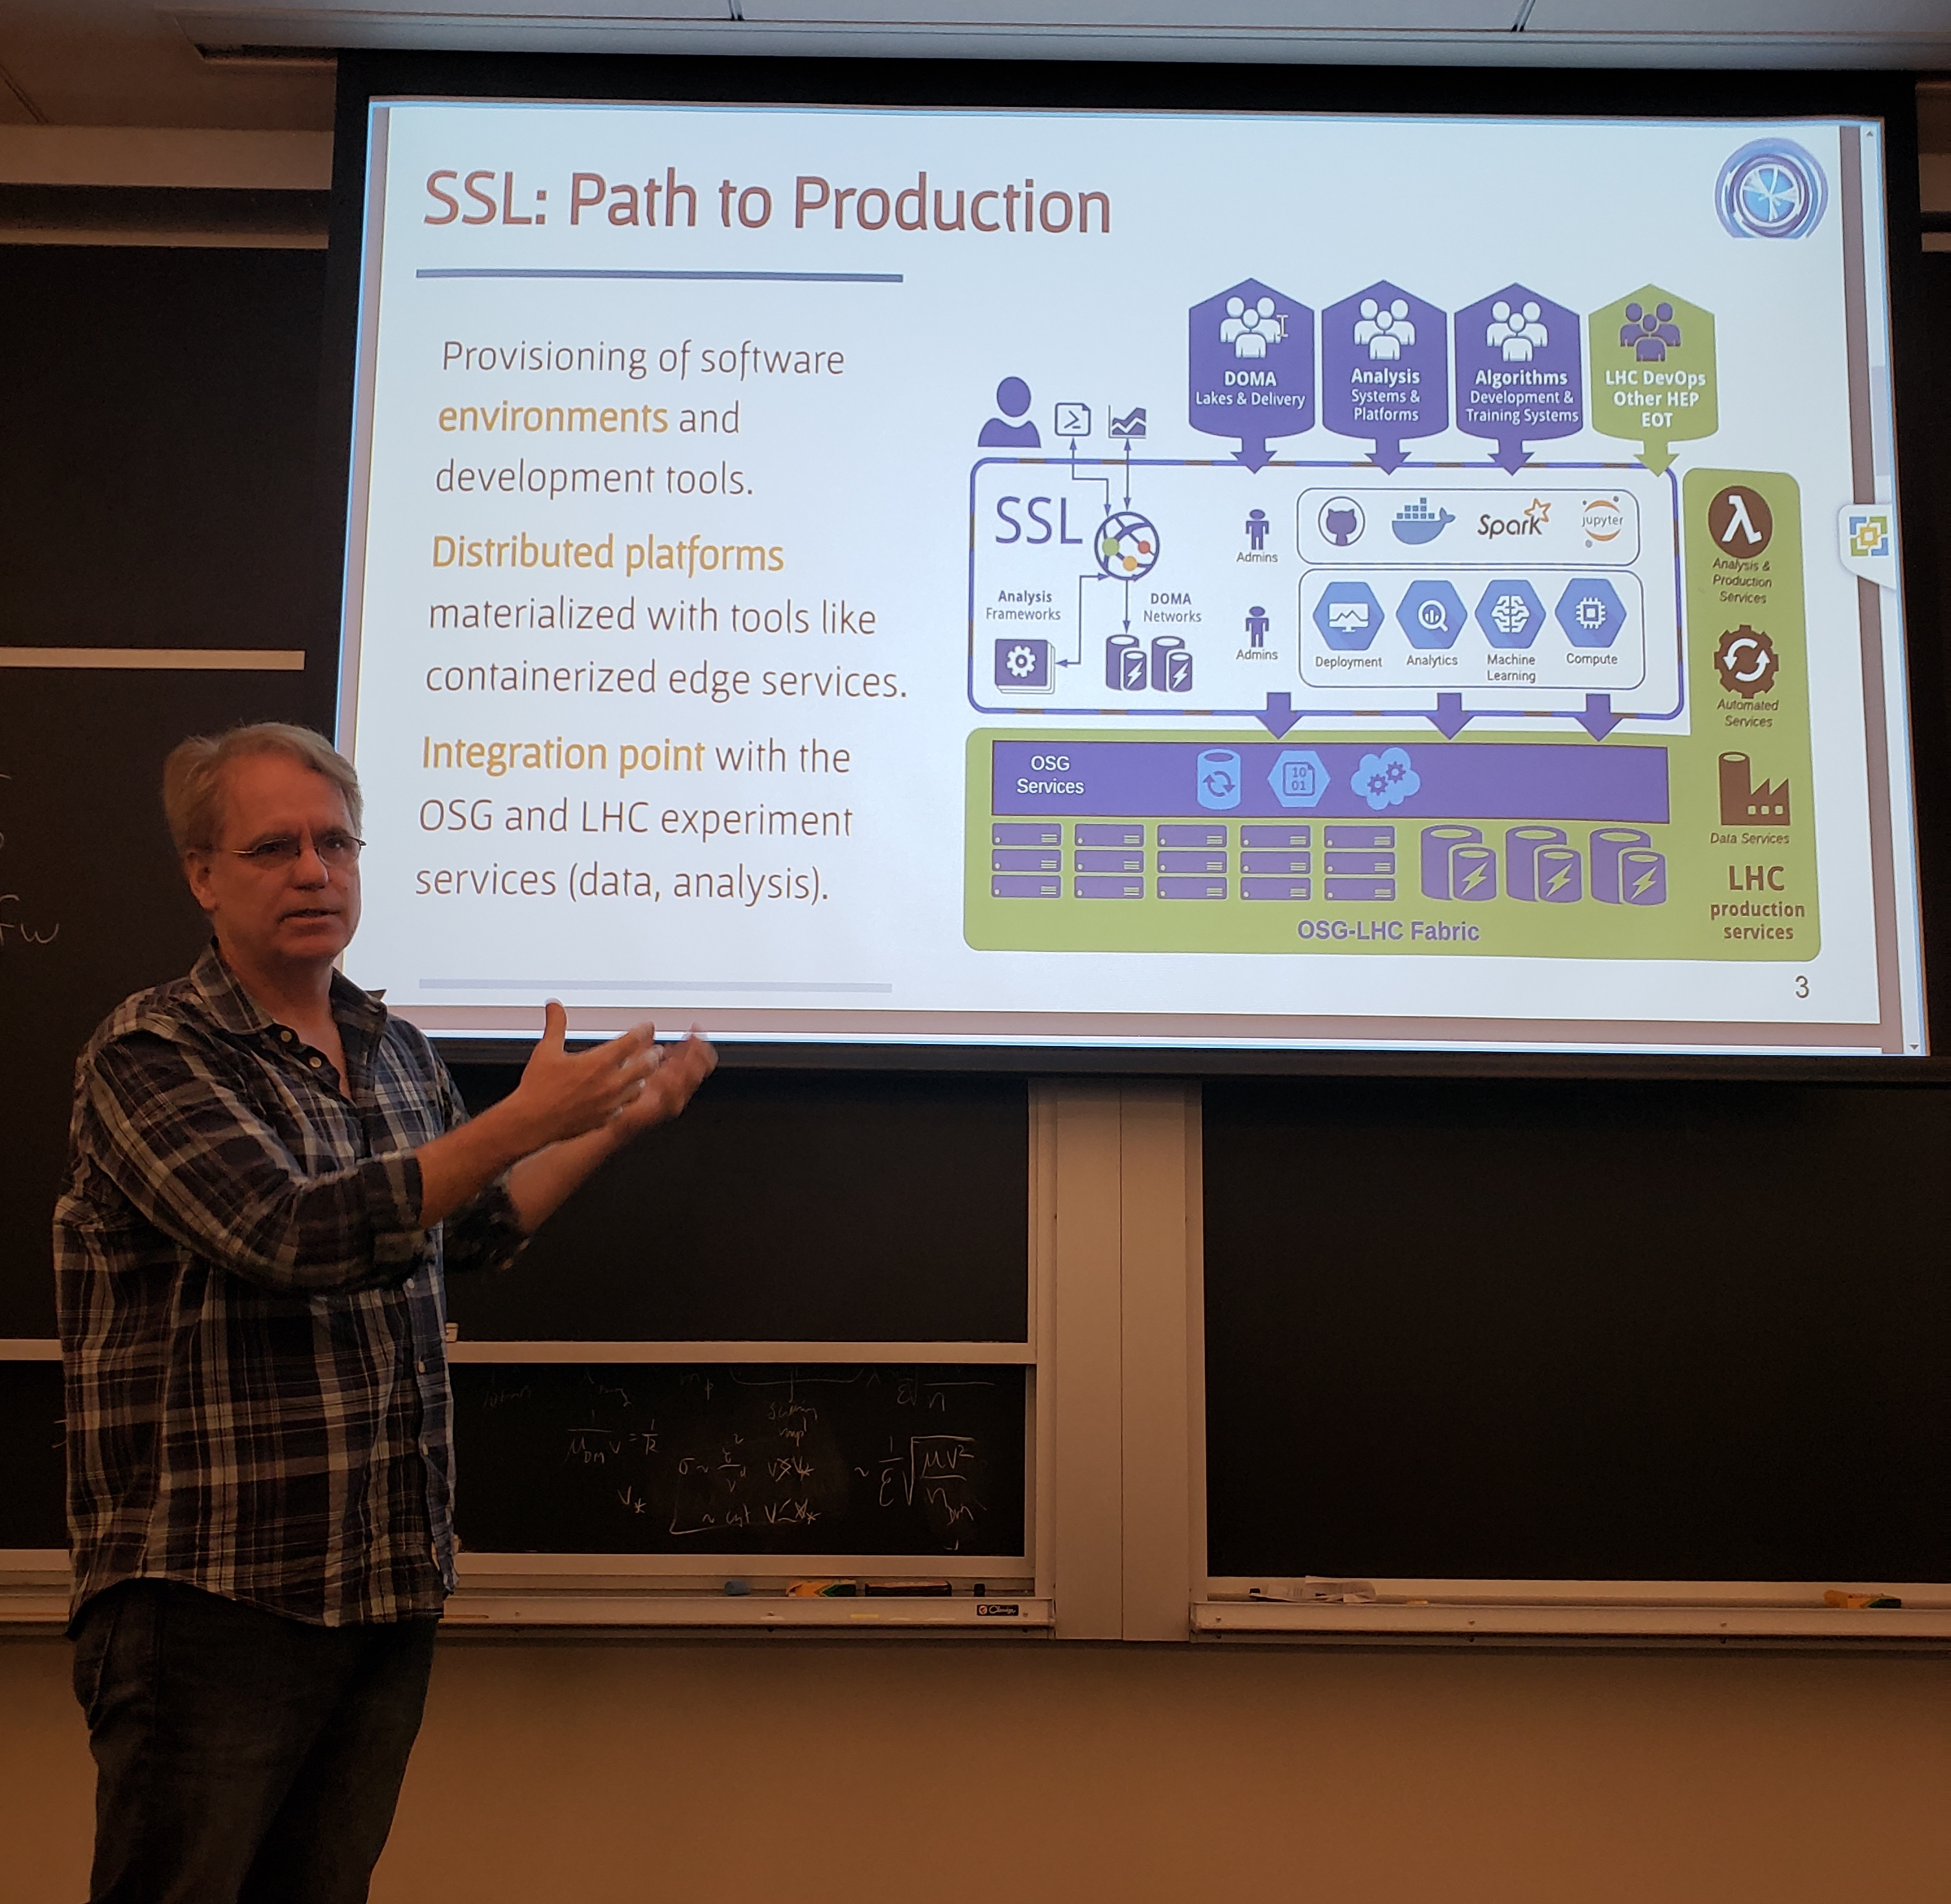
\includegraphics[width=0.99\linewidth]{figures/rwg_ssl.jpg}
  \vspace{-0.7cm}
  \caption{Rob Gardner (Chicago) presents on the SSL concept on Day 1 of the workshop.}
  \label{fig:rwg_ssl}
\end{wrapfigure}
(at the time of writing) the SSL core has less than one FTE of funded effort, success will depend critically on leveraging efforts from other areas of IRIS-HEP and engaged partners. The high-level purpose of the SSL is to provide the Institute and the HL-LHC experiments with scalable platforms needed for development in context, i.e. the {\textit path to production} use within the experiments, as illustrated in Figure~\ref{fig:overview}.

As presented in Section~\ref{sec:Goals}, one of the goals of the AS/SSL Blueprint workshop was to further develop the SSL concept, scope and architecture. These were presented in Gardner's talk and informed by the subsequent discussions at the workshop. The SSL will be designed to:
\begin{itemize}
  \item Provide access to software and computing infrastructure and environments
  \item Organize software and resources for scalability testing
  \item Provide foundational systems R\&D on accelerated services
  \item Provide the integration path to the production infrastructure of the experiments
\end{itemize}
The SSL elements and role within IRIS-HEP and broader ecosystem are shown in Figure~\ref{fig:ssl}.

Among the challenges for SSL is that it must be a community platform across numerous experiments and institutions -- it should support groups (and projects) with specific organizational membership for access to resources with the appropriate level of permission. It must aggregate {\it bespoke} resources and configurations and do so in a {\it declarative} fashion such that deployments are reproducible and {\it mobile}. It must provide services to build and manage deployment artifacts. Finally, it must be scalable up and down as testing activities are episodic in nature.

The opportunities presented to the community are that in building out the SSL, \textit{ad-hoc} collaborations will be formed which cross organizational boundaries; contributions will come from diverse resource providers, broadening participation; new models of infrastructure development will be discovered supporting more rapid innovation of analysis systems; and that having catalogs of service artifacts capable of patterned re-deployments in open, robust orchestration systems should accelerate delivery of R\&D products for use in production.

\begin{figure}[ht!]
  \centering
  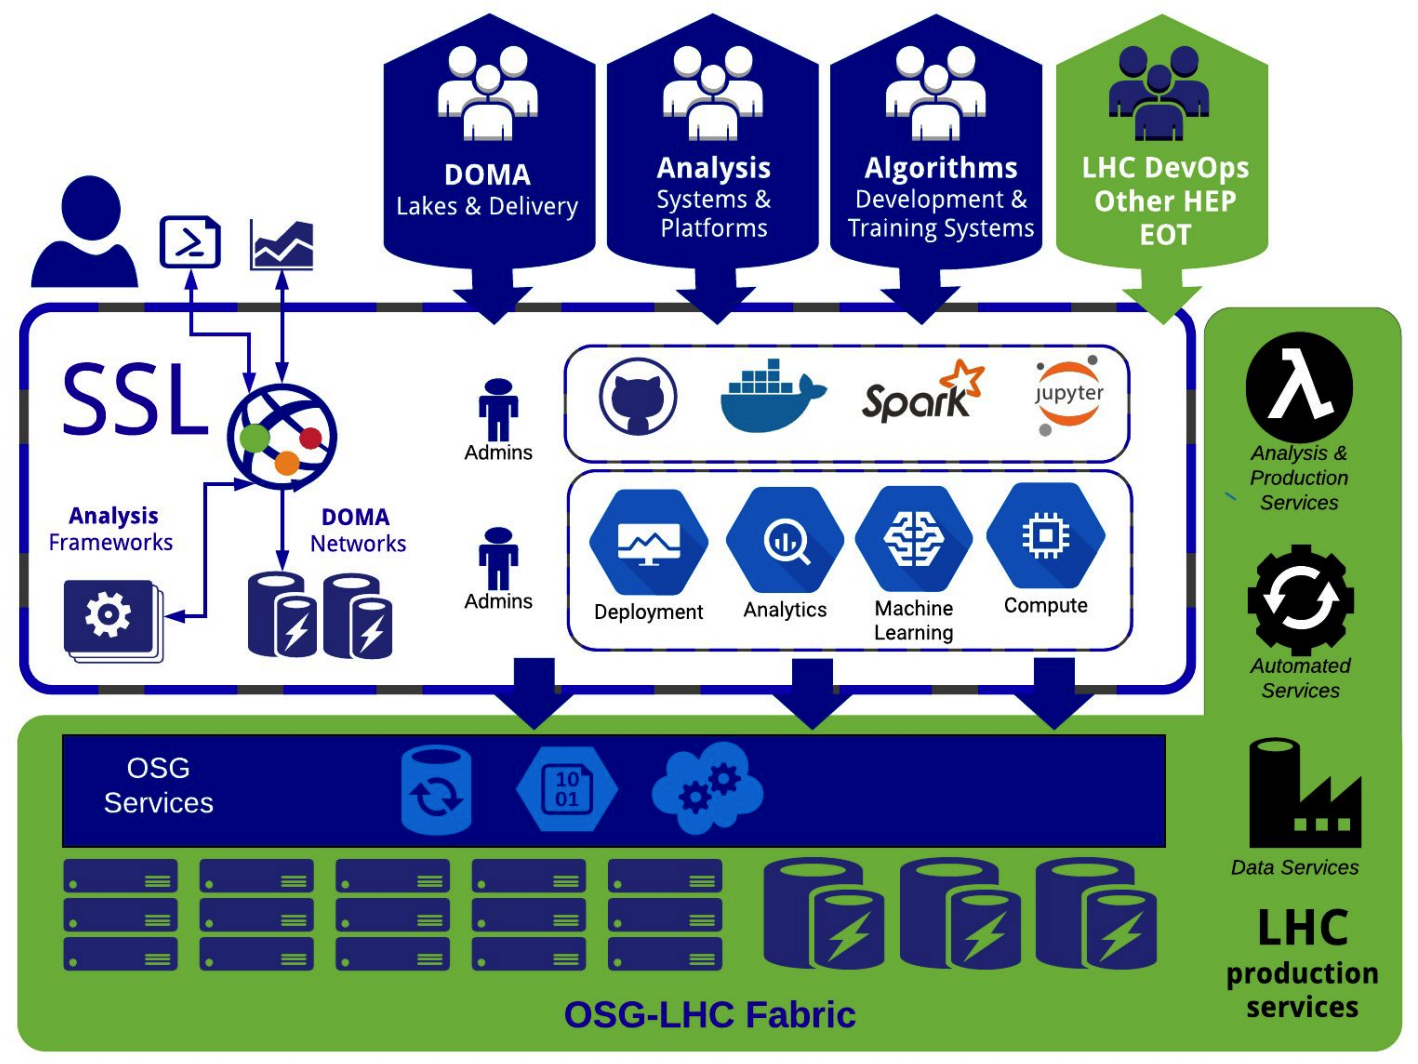
\includegraphics[width=0.99\linewidth]{figures/ssl.png}
  \vspace{-0.3cm}
  \caption{Schematic diagram of SSL elements and role within IRIS-HEP and broader ecosystem.}
  \label{fig:ssl}
\end{figure}

It was noted that storage, processing and networking become significant challenges for the relevant scale testing needed, and so the following question arises: \textit{how does the SSL provision accordingly?} The possibility of augmenting existing on-premise resources with public cloud was discussed, with examples cited such as a recent million core-scale computation by an MIT researcher. This led to a general discussion of cost comparisons between institutional providers and public cloud. It was agreed with any test all options should be considered and costs periodically assessed. Additionally, research partnerships where there is mutual interest with public cloud providers should continue to be exploited. Finally, it was noted that specifics of the server/instance targets need to be considered, such as memory-per-core and I/O bandwidth which could pose special challenges and associated costs.

\subsubsection{Analysis Systems}
\vspace{0.2cm}
Kyle Cranmer (NYU) presented \href{https://indico.cern.ch/event/820946/contributions/3461589/attachments/1867063/3070546/AS-SSL-Blueprint.pdf}{\textit{Analysis Systems Perspectives \& Goals}}. The \href{https://indico.cern.ch/event/822074/}{Analysis Systems Topic Workshop} completed the day prior to the start of the Blueprint workshop revisited the milestones and deliverables for the rest of IRIS-HEP Year 1 and and Year 2 planning. It was noted there are AS scalbility milestones in Y2Q1 which imply specific requirements on SSL readiness. The goal that developed was to move testing onto whatever resources are currently in use to an \textit{SSL-managed} infrastructure. This includes prototypes of analysis systems components to be deployed on the SSL by August 2020.

There were notable ad hoc demos of interest to the workshop. First was the {\sf REANA}/{\sf RECAST} demo at \href{https://kccna18.sched.com}{KubeCon 2018}, focusing on reproducibility of a real LHC analysis, demonstrated that HEP can engage with modern open source tools and communities. Second was the scalability demo of Higgs rediscovery on Kubernetes (200 GB/s, 70 TB) performed at \href{https://events.linuxfoundation.org/events/kubecon-cloudnativecon-europe-2019/}{KubeCon and CloudNativeCon Europe 2019}. There are other examples in our field, e.g. \href{https://www.youtube.com/watch?v=Ye8MlJQumaI}{\textit {CERN’s Next Generation Data Analysis Platform with Apache Spark}} by Enric Tejedor (CERN) at the \href{https://databricks.com/sparkaisummit/europe?utm_source=google&utm_medium=cpc&utm_campaign=g_s_brand_beta&gclid=EAIaIQobChMIhO7fksjC5AIVDRgMCh0kFwcaEAAYASAAEgKjSPD_BwE}{Spark+AI Summit Europe in London, October 2018.}

A number of systems under development have or will soon emerge from AS that are candidates for deployment and testing on the SSL.
\begin{itemize}
  \item \textbf{\textit{ServiceX}}: Part of DOMA's efforts to develop the intelligent data delivery services (IDDS), the service focuses on reformatting data a the end-stage analysis phase, transforming event data into columnar formats which provide advantages for effciency and Python-based processing frameworks.
  \item \textbf{\textit{Coffea}}: A columnar analysis framework being developed at Fermilab. It was noted at the workshop that soon there are ServiceX + Coffea demonstrators.
  \item \textbf{\textit{MadMiner}}: Containerized workflows with mix of CPU and GPU/TPU acceleration, toward the integration of simulation, machine learning, and statistical inference to reduce time-to-insight. These workflows are ready for execution on Kubernetes using {\sf REANA} and identified as primary candidates to exercise analysis systems technologies and infrastructurre for physics.
  \item \textbf{\textit{AMPGEN}} \& \textbf{\textit{pyhf}}: Tools under development toward system(s) that provide fitting-as-a-service to HEP physicists. Have resources setup and available for users to upload statistics "workspace" information (e.g., pyhf JSON) and then the service performs the fits; providing the best-fit parameters, covariances, goodness-of-fit estimates, etc. Such a service will provide mechanisms to optimize inference acceleration (GPUs, etc) and will save the user from having to set things up on their own -- services are simple, but not everyone has a nice GPU cluster on the backend ready to go.
\end{itemize}

The types of systems the AS team has considered for development and testing were discussed. These types incluced public cloud (speed of startup, additional services), university resources (on-premisis costs, data storage), existing grid infrastructure (e.g. the Open Science Grid) which has a dedicated integration team (OSG-LHC) within IRIS-HEP, and DOE and NSF leadership class HPC systems. The importance of having the ability to move service deployments and workloads between these resource categories was noted.

The role of container usage on the grid was discussed, including early applications in distributed training (e.g. hyperparameter tuning).  Much existing work can be leveraged here, with previous efforts reported at \href{https://indico.cern.ch/event/708041/}{ACAT 2019}, and talks on machine learning in ATLAS using Docker images.

The possiblity of providing HPC "backends" to {\sf REANA}, including HPC, was discussed and considered a worthy goal. An interesting side topic was the emerging market of resources for machine learning outside the public cloud providers and HPC centers; in particular \href{Vast.ai}{vast.ai} provides a cloud computing, matchmaking and aggregation service focused on lowering the price of compute-intensive workloads.

\subsubsection{SSL Architectural Principles}
\vspace{0.2cm}
Lincoln Bryant (Chicago) presented \href{https://indico.cern.ch/event/820946/contributions/3461592/attachments/1866998/3119402/2019.06.21_SSL_Patterns__Deployments_Lincoln.pdf}{\textit{SSL Hybrid Models, Developer Support \& Deployments}}. There are a number of desirable features that have been identified for the SSL.  These include community access - open to all working on software infrastructure in HEP - which can be implemented with federation tools based on {\sf CI-Logon}, for example, providing a single sign-on capability; a lightweight group (project) management system; infrastructure itself should be \textit{composable and reusable}; being able to accommodate and aggregate a diverse resource pool and user community; a container-based service orchestration on dedicated resources; \href{http://www.virtualclusters.org/}{VC3}-like technology to connect to HPC/HTC resources for batch scale-out; and facilitate integration of commercial cloud resources when needed.

Regarding declarative and reproducible deployments, the goal is to have infrastructure built under the SSL to be easily reusable and deployable to other sites. In short, we require the SSL to provide resources that are \textit{discoverable}, \textit{flexible}, and \textit{nimble}. The declarative nature of Kubernetes is a good fit to the SSL requirments and gets us a long way to providing such a service.

The SSL itself is \textit{not} intended to become a \textit{production center}. Rather, it should serve as an \textit{incubator} for projects which then \textit{graduate} to become a full-fledged infrastructures that run on production resources. Services to build and manage artifacts -- tools that provide SSL to be scaled up and then back down are part of reducing cognitive load for developers and deployers.

The SSL team is currently using Google's Kubernetes Engine -- the \href{https://cloud.google.com}{Google Cloud Platform} (GCP) - to test ServiceX deployment; this will soon be pulled off GCP and into in-house resources running on Kubernates and integrated into the SSL.

From the university point of view, groups that want to deploy and validate AS systems locally should be empowered with the resources required to have simple versions of what these systems need to provide -- for example, a base Kubernetes cluster and a functional {\sf REANA} instance -- as a start. From a campus IT/research technology point of view, easy to deploy systems offer the ability to make a compelling case to campus administration that they are providing resources whcich enable good science.

There were some lightweight mechanisms suggested for discovery of resources.   The value of reporting and showing science that is happening on the contributed resources to incentivize resource providers at the universities was noted.  Capturing success stories, so university community understands how they can benefit from investments to shared campus resources, including staff, were discussed. Having a dashboard may help visualize and communicate the contributions groups are providing to IRIS-HEP through SSL. This would be important for products that can be used outside HEP, ultimately giving them higher visibility within the broader community.

There were questions as to whether the SSL provisioning method, dashboard panels, and other tools developed to materialize and manage the service infrasructure would be open sourced and productized. These were interesting possibilities and would depend on the level of effort available and a balancing of other priorities.

\subsubsection{Experience with Google Cloud Platform}
\vspace{0.2cm}
Lukas Heinrich (CERN) presented \href{https://indico.cern.ch/event/820946/contributions/3461593/attachments/1867157/3070768/go}{\textit{Use of the Google Cloud Platform in High-Energy Physics}}. The KubeCon 2019 keynote \href{https://sched.co/MRyv}{Reperforming a Nobel Prize Discovery on Kubernetes} was illustrative of the power and flexibility of Kubernetes and its relevance the HEP computing. The CMS open data sample (70 TB, 25000 files) was reprocessed on live on stage using legacy software from the CMS scientific software stack and Kubernetes at a large scale. The main lessons learned were that the Google Network can serve extreme data rates into compute nodes (2 Gbps/core) once handled appropriately. Incoming data could be staged using Google tools but disks that can handle the required rates (e.g. local SSD drives) are scarce. A write-to-memory scheme was therefore developed. At highly parallel workloads, scheduling become very important and these systems are still undeveloped in Kubernetes.

\subsubsection{Easing Kubernetes Deployment}
\vspace{0.2cm}
Sanjay Arora (RedHat) presented \href{https://indico.cern.ch/event/820946/contributions/3461594/attachments/1867161/3070777/OpenShift_4.pdf}{\textit{RedHat OpenShift}}. \href{https://www.openshift.com/}{OpenShift} is distribution of Kubernetes that makes on-premisis clusters easier to deploy and maintain. The model is analogous to RedHat's release of Linux, and there is an open source equivalent to {\sf CentOS} for OpenShift: \href{https://www.okd.io/}{OKD}. If Kubernetes is to play a central role in a re-engineered WLCG computing infrastructure, its distribution and management could benefit from solutions such as these and similar technologies.

\subsubsection{Perspectives from University Resource Providers}
\vspace{0.2cm}
David Ackerman (CIO, NYU) presented \href{https://indico.cern.ch/event/820946/contributions/3461596/attachments/1867159/3070772/go}{\textit{Research Computing Technology at NYU}}. In this talk, some of the recent activities and exiting plans for research computing at NYU were presented. Notable, a low-latency, high-throughput research network is under development which has interesting connections to the R\&D work being done in the AS area within IRIS-HEP.

\subsubsection{Google Perspective}
\vspace{0.2cm}
Stephan Fang (Google) presented \href{https://indico.cern.ch/event/820946/contributions/3461593/attachments/1867157/3070794/go}{\textit{Google Perspective}}. Stephan's talk (see Figure~\ref{fig:google}) sparked an \begin{wrapfigure}[16]{R}{0.48\textwidth}
  \vspace{-0.4cm}
  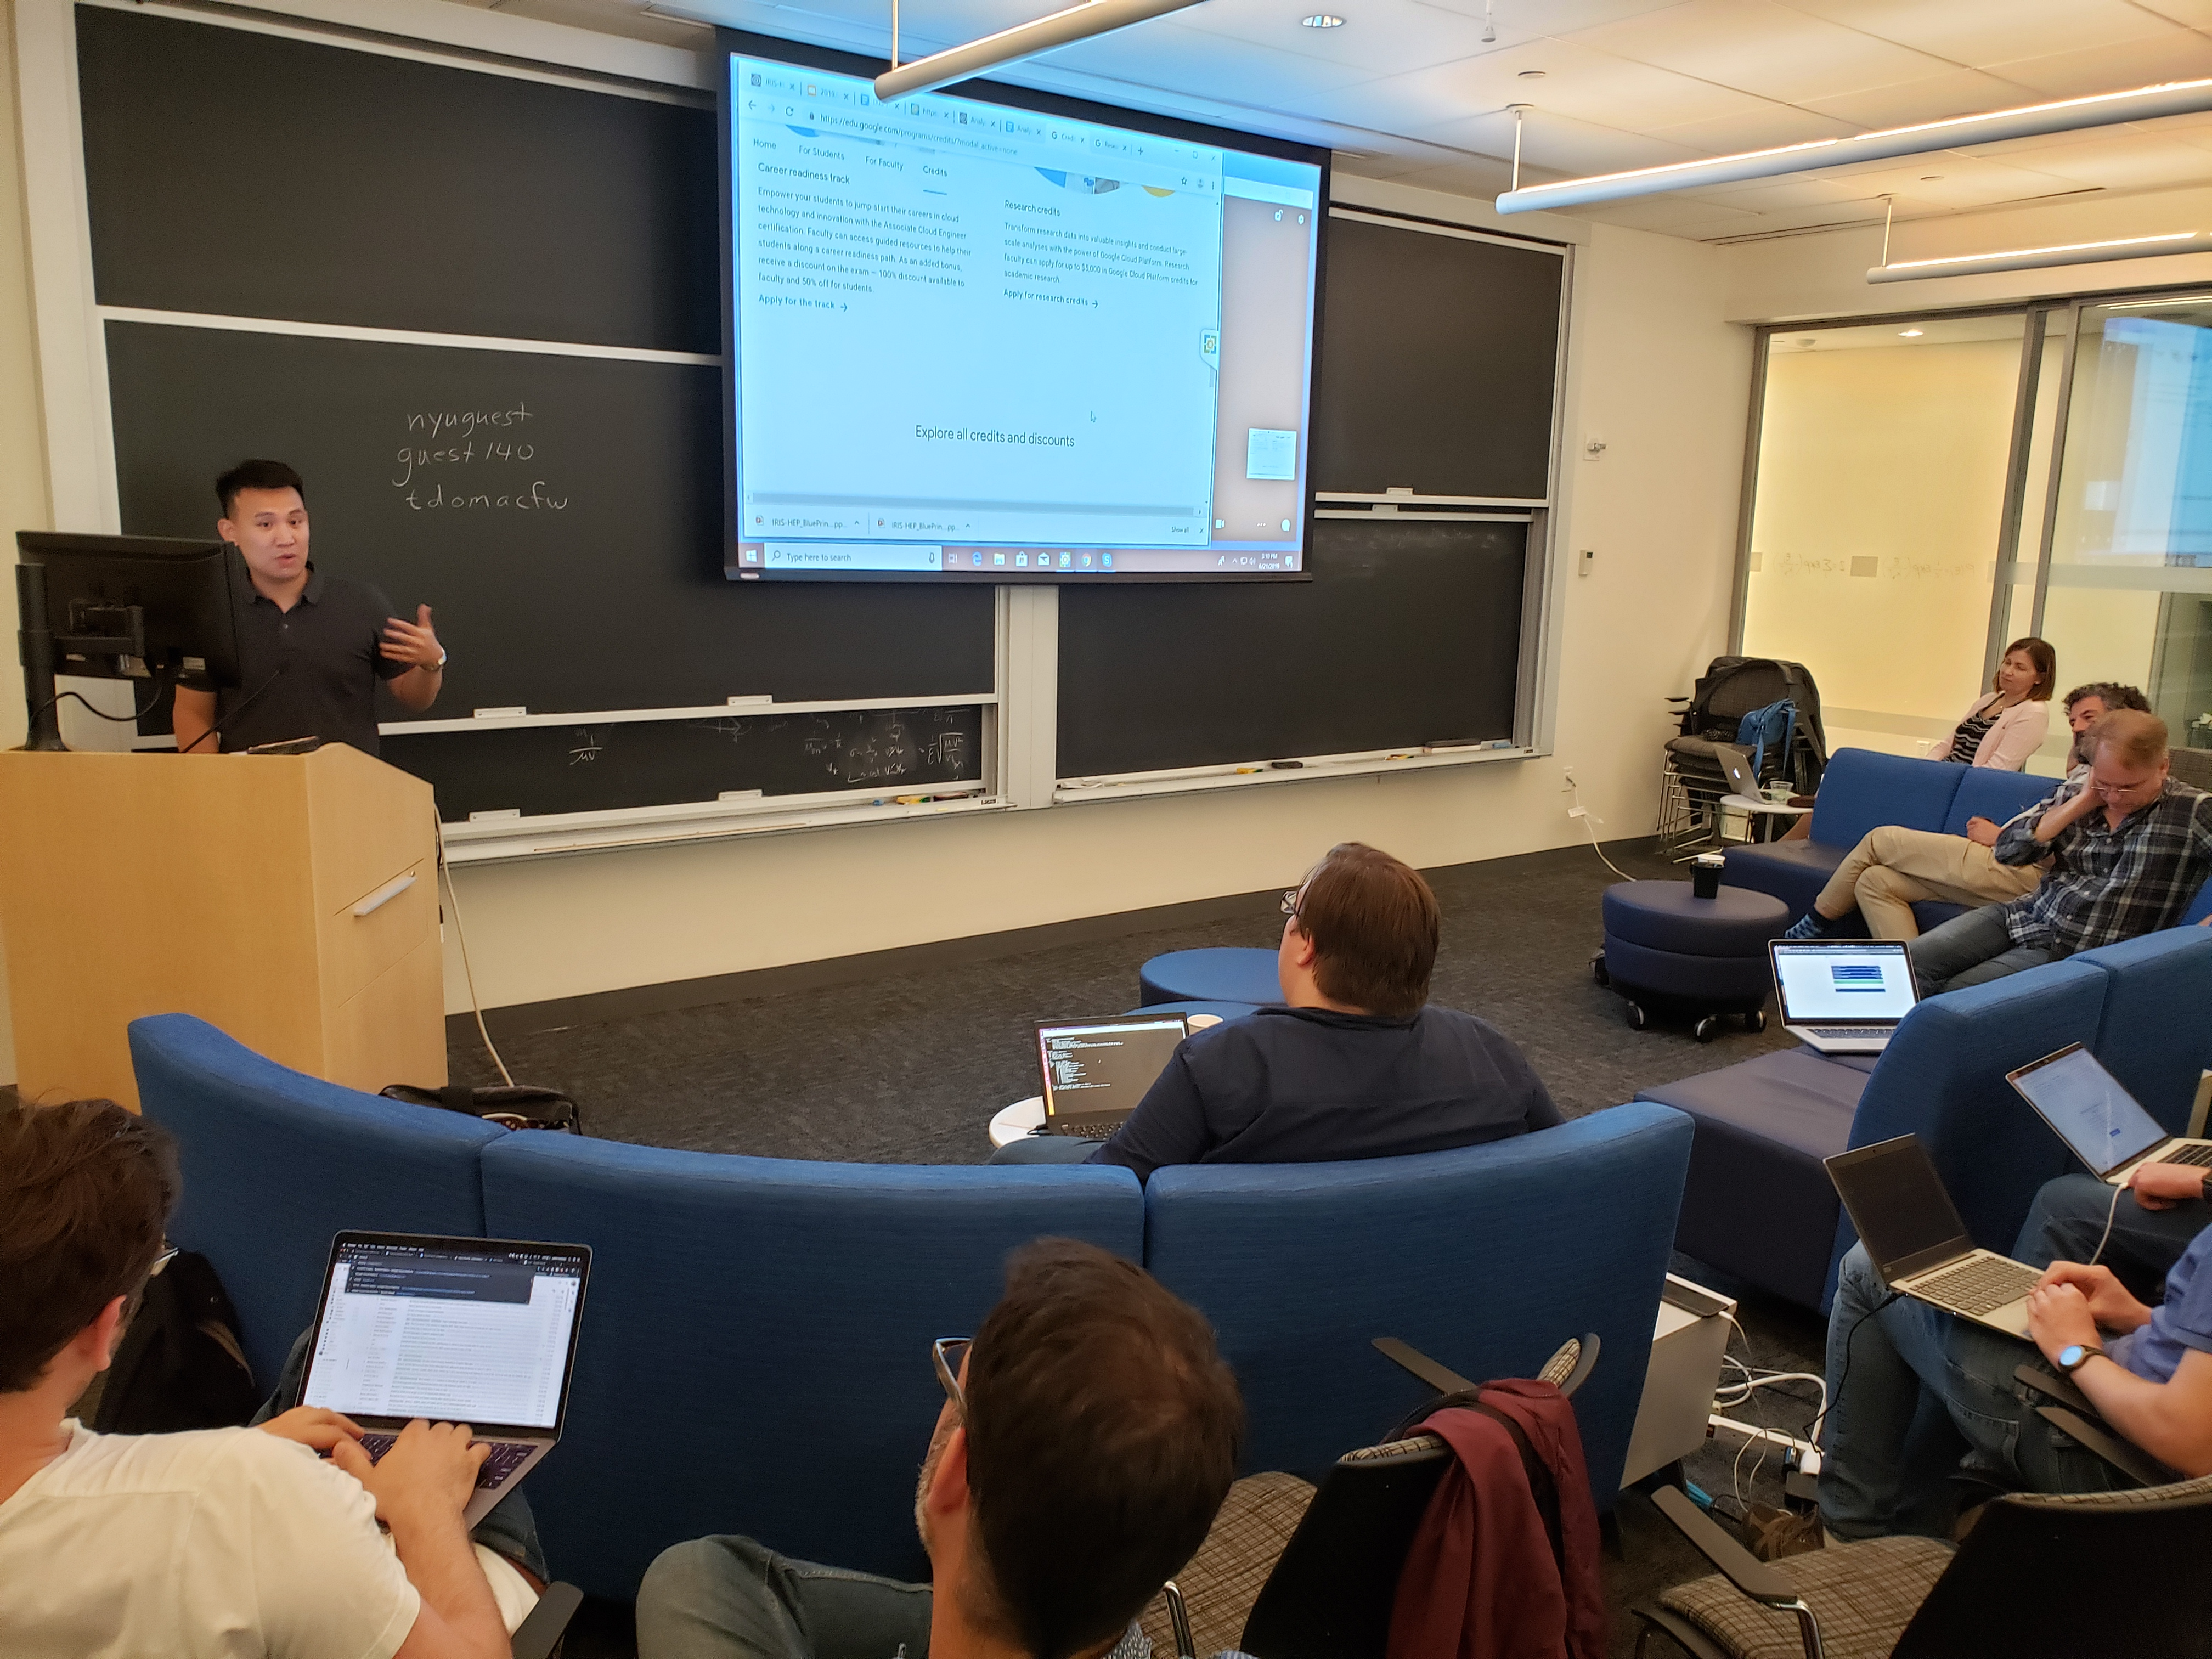
\includegraphics[width=0.99\linewidth]{figures/google.jpg}
  \vspace{-0.7cm}
  \caption{Stephen Fang (Google) presents on Google perspective about data analytics and education at the workshop.}
  \label{fig:google}
\end{wrapfigure}
interesting and productive discussion at the workshop about how the proposed fitting service within AS is well-aligned (e.g. pyhf) with the use of Google cloud credits and interest in the use of GPUs and TPUs for benchmarking and scaling studies. Stephen mentioned that there is a TPU research group and that this team collaborates with researches to optimize systems for TPUs. The plan discussed at the meeting was for activity to be coordinated under SSL and to have a prototype system for TPU benchmarking by December 2019.

Stephen also discussed the
\href{https://edu.google.com/programs/credits/?modal_active=none}{researcher credit program for education} and some attendees of the workshop mentioned that they are either teaching or developing courses in data analysis and machine learning that could benefit from such engagement.

\subsubsection{Accelerated Systems}
\vspace{0.2cm}
Andrew Chien (Chicago) presented \href{https://indico.cern.ch/event/820946/contributions/3464565/attachments/1867166/3070786/IRIS-HEP-Accelerated-Scalability-6-21-2019-v2.pdf}{\textit{Accelerated Systems \& Optimization}}.  System scalability research within computer sciene offers an opportunity to optimize the use of resources in specific areas in an end-to-end computing system. For a local database, it is all about query optimization with predicates and filters; by exploiting selectivity one can increase the scalability and performance of a system. In a public cloud context, services such as \href{https://aws.amazon.com/blogs/aws/s3-glacier-select/}{AWS S3 Select} offer the ability to accelerate services through partial selection of objects before delivery to clients. Opportunities in HEP include (optionally hardware) filtering in strategic locations to reduce traffic on the wide area network for data delivery. Previous findings on studies of data transformation with recoding accelerators, with programmable accelerators allowing the right representation choice (and format) performed in the {\it right place} have potential for cheaper computation, less data movement and higher performance.

Throughout the presentation a number of \textit{dimensions of benefit} involving system optimization choices with acceleration were identified:
\begin{itemize}
  \item Reduction in parsing \& filtering costs (through acceleration)
  \item Performance through more aggressive query optimization
  \item Representation of encoding in Query Execution Plan
  \item Beyond tuples to block/transpose, special recoding (ex. ML inference and analysis for systems), etc.
  \item Exposing new optimizations to eliminate transformation overhead
  \item Reduction in CPU load through off-loaded computation, reducing total data processed
  \item Shifting of Filtering computation to Storage nodes
  \item Reduction in Data Center network load
\end{itemize}

\subsection{Afternoon Discussion}
\vspace{0.2cm}
In thinking of concrete progress for AS-SSL activities, \href{http://www.reanahub.io/}{REANA} was identified as a good first deployment target for the SSL. In addition, ServiceX as deployed on Google Cloud Platform via Helm would make it an interesting use case if the SSL API is Kubernetes.

We discussed a {\sf REANA} instance deployed on an SSL cluster provisioned with OpenShift. Success of the deployment would be to have two independent sets of people deploy and succesfully run the example provided. Templated python scripts, HELM charts, and YAML would be the ingredients. The question of what would be needed from the SSL to accomplish this was discussed, finding that SSL needs to provide:
\begin{itemize}
  \item Storage
  \item Internet ingress
  \item Load balancing
  \item Pod capacity
\end{itemize}

Other questions arose, for example whether or not there is one SSL (as a service) or a reference standard. As a pattern, we would like not to have a site administrator having to follow notes off a Twiki page to stand up Kubernetes. Instead, we would like the admin to connect their nodes to an SSL console and everything is automatically deployed. The process to join must be lightweight otherwise it will be difficult to maintain productive partnership with those providing SSL resources. If one observes a deployed pattern, they should be able to deploy the pattern to a local environment.

As a users of SSL, one should at a minimim publish deployment instructions so others can reproduce it. In some respects, this like an R\&D Hybrid Cloud provider. SSL should try to make any service substrate as compatible as possible with CERN-IT, FermiLab and other national laboratories.

A question was put forward regarding possible blockers to this approach of using Kubernates: \textit{if a federated set of Kubernetes clusters is the substrated approach for SSL, do we lose anything regarding AS R\&D on SSL?} The answer for AS was that there does not seem to be blockers, but HPC integration might need further consideration to ensure that this is not the case. For scaling tests, federating SSL clusters would be very desirable for facilitating this activity.

{\bf Metric data} would be useful to have from SSL. Dashboards and retention of results, the ability to mine metadata indexed by ElasticSearch, use of Kubernetes monitors such as Prometheus would provide some of this.  Developing the complete suite for logging and metrics collection is out of scope of SSL, but maybe provide a few standard tools and a repository to collect notes on best practice.

There were comments that not everyone in our group knows how to build a Helm chart -- the \textit{de facto} standard for Kubernetes deployments at this time. While that is certainly true currenly, the majority of projects AS is working on is going to fit into a Helm chart eventually - so there is something to be said for being able to use it for early examples. Docker/desktop can run kubernetes and it is not yet known how hard it is to make a flexible Helm chart which can scale from a single node cluster to many nodes and clusters, but this means that the person working on the component can basically run it in the environment they will eventually have to run in. Generally it was agreed the burden would be to the R\&D areas to define the metrics and guide SSL on what data to retain.

We discussed SSL {\bf service Level agreements} between research teams and the SSL; their role and utility for setting developer and resource provider expectations.  Some ideas included agreement to publish deployment artifacts, ability to request time and scheduling for scalability tests, and agreement on the needed information before devoting significant resources to such an activity.

Opportunities and planning for SSL resources were discussed. For example, should there be regions of the SSL where clusters nearby are logically group or technically joined via a federation or mesh software? It was agreed that successful contributins would rely on tools that allow operators the ability to re-create SSL environments at another location. Specific initial sites discussed included:
\begin{itemize}
  \item NCSA: \href{http://www.ncsa.illinois.edu/about/org/isl}{the Innovative Systems Laboratory (ISL)}, the Openstack cluster, \href{http://www.ncsa.illinois.edu/enabling/bluewaters}{the Blue Waters supercomputer}, the \href{https://campuscluster.illinois.edu}{Illinois Campus Cluster} (an ATLAS Tier-2 provider with opportunistic use of CPUs and GPUs), and an NSF MRI \href{https://wiki.ncsa.illinois.edu/display/ISL20/HAL+cluster}{Deep Learning research platform (HAL)}.
  \item Redhat (Openshift) - there is the Massachusetts Open Cloud
  \item CERN
  \item NYU
  \item Fermilab
  \item BNL
  \item SDSC and the Pacific Research Platform
\end{itemize}

\subsection{Day 2 Breakout Session}
\vspace{0.2cm}
On the second day, participants broke into two (roughly equal) groups for more detailed discussion and development of the key workshop outcomes and action items. One group examined specific issues related requirements from the Year 2 plan for AS. The second group assembled to discuss topics around SSL infrastructure and to identify an impactful path moving forward. The assignment of which participants were in which group was voluntary based on interests of each participant.

\subsubsection{Analysis Systems Breakout}
\vspace{0.2cm}
The AS breakout session was lead by Kyle Cranmer who began with a presentation of the milestones, as shown in Figure~\ref{fig:AS_milestones}.
\begin{figure}
  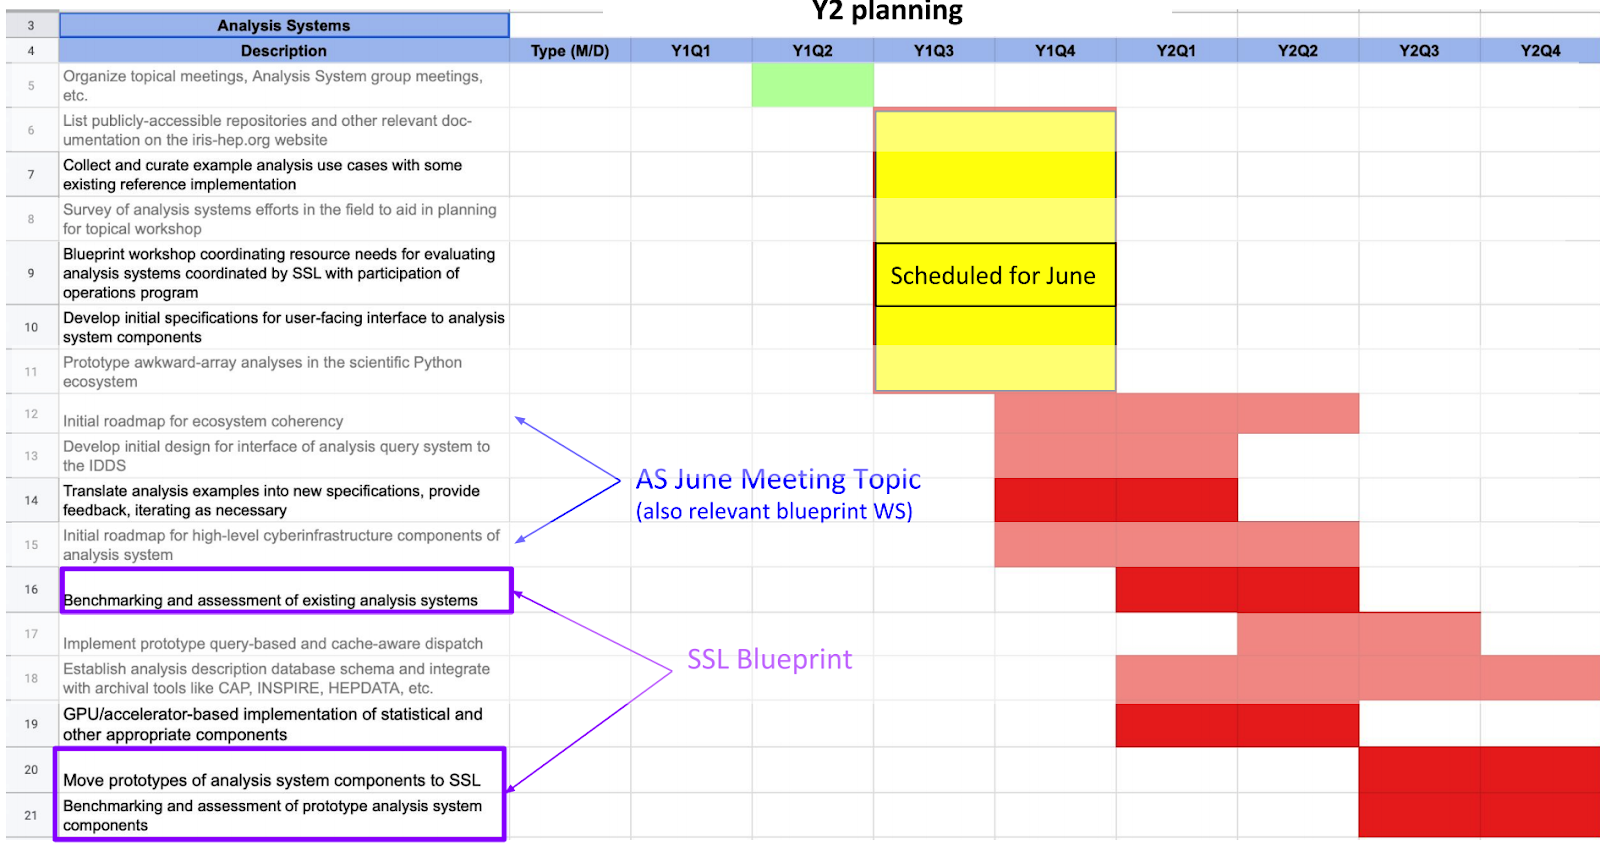
\includegraphics[width=\linewidth]{figures/as_milestones.png}
  \caption{Annotated snapshot of the AS milestones presented in the AS breakout session on Day 2 of the workshop.}
  \label{fig:AS_milestones}
\end{figure}
The following discussion focused on answering the following question: {\it What SSL cyberinfrastructure is required for AS success?}. Key elements that were put forward during the discussion included:
\begin{itemize}
  \item {\it Lowering barriers for participation in analysis systems} that are currently under development. This includes clear and thorough documentation, particularly the devalopment and maintenance of workuing examples
  \item {\it Empowering small groups with limited physical infrastructure and personnel to contribute meaningfully to data analysis}. There are growing concerns within the HEP communitiy that it is becoming increasingly difficult for single-PI groups to make a strong impact to physics papers on the large experiments. This issue is on the radar screen of the agencies as well and touches on challenges around diversity and outreach. It was pointed out that one way to address this challenge is to streamline the process of onboarding and transfer ("forward evolution") of analyses. As an example, RECAST represented a new style of doing analysis which CERN cloud servies facilitated. Similarly, there are \href{https://gitlab.cern.ch/aml/containers/docker}{ATLAS base Docker images} for machine learning. If SSL can provide these types of services quickly it would move forward critically-needed developments in this area.
  \item {\it Establishing mechanisms for SSL to coordinate with campus IT efforts to replicate working environments} For example, NYU and k8 research clusters were proposed to test this paradigm. This activity could also inform the future evolution of the Tier-2s. It was commented that Openshift is popular in large part becuase it makes Kubernates easy to deploy and work (and that CVMFS works on Kubernates)
  \item {\it SSL as a matchmaker and hub for relationships} of analyzers and developers.
  \item {\it BinderHub connected to SSL authentication} as one of the capabilities in the SSL service catalogue. A
  \href{https://mybinder.org/}{Binder} example is the \href{https://mybinder.org/v2/gh/diana-hep/pyhf/master?filepath=docs%2Fexamples%2Fnotebooks%2Fbinderexample%2FStatisticalAnalysis.ipynb}{pyhf example stat analysis}.

\end{itemize}

\subsubsection{SSL Infrastructure Breakout}
\vspace{0.2cm}
The SSL Infrastructure breakout session was lead by Rob Gardner who began with a discussion of the Y1Q4/Y2 SSL milestones and development of an SSL roadmap, which included: \\
Y1Q4
\begin{itemize}
  \item Roadmap of initial cyberinfrastructure components from AS.
  \item SSL substrate project (see below)
  \item REANA service deployed (with HELM charts)
  \item ServiceX deployed (gke->ssl procedure defined)
\end{itemize}
Y2Q1
\begin{itemize}
  \item A general app monitoring, benchmarking, metrics collection service
  \item A model for next generation Tier2s \& Tier3s
  \item HEPIX, Oct 14-18: https://indico.cern.ch/event/810635/abstracts/
  \item Presentation at CHEP
\end{itemize}
Y2Q2
\begin{itemize}
  \item Further engagement with SSL clients, including reservation scheduling
\end{itemize}

\vspace{0.1cm}\noindent
\textit{\underline{SSL Substrate Project}} \\
A key idea developed at the workshop was to deploy SSL resources as set of clusters based on kubernetes. In this way, various contanerized SSL applications could be deployed on SSL resources in a flexible and nimble manner. The first step is deploy a set of kubernetes clusters ("substrate") that participate in SSL - i.e. build out a thin k8s substrate layer from contributed resources.

Proposed partners (with contact persons) include
\begin{itemize}
  \item Chicago (River - Lincoln/Andrew)
  \item Illinois (Illinois Campus Cluster (ICC) - Tim Borner)
  \item New York (legacy T3 \& research tech’s k8 cluster)
  \item San Diego (campus k8s + PRP + UCIrvine - Edgar)
  \item CERN (coordinate with existing patterns and successes)
  \item Princeton (to be developed)
  \item Fermilab (Glen Cooper, Liz, … to be developed)
  \item BNL (to be developed, challenges)
\end{itemize}

\section{Key Outcomes and Action Items}
\vspace{0.2cm}
Below summarize the key outcomes of the workshop:
\begin{itemize}
  \item Communication of the AS area plans and a preliminary set of requirements to SSL team.
  \item Kubernetes identified as a planned {\it common denominator} technology for the SSL, increasing innovation capability through flexible infrastructure.  This idea spawned plans for a multi-site SSL {\it substrate} project that will federate SSL contributions from multiple resource providers (institutes and public cloud), offering the AS area a flexible platform for service deployment at scales needed to test the viability of system designs.
  \item Productive engagement of the AS/SSL team with representatives from NCSA, SDSC, NYU Research Computing, industry \& cloud providers (Google, Redhat), generating action items and informing Year 2 planning of IRIS-HEP.
  \item A concrete vision for an SSL that serves not only as an innovation space for AS developers, but as a testbed to prototype next generation infrastructure patterns for future HEP computing environments.
\end{itemize}
There were a number of action items generated by the breakout sessions, among them are:
\begin{enumerate}
  \item Deploy an AS validator application on the initial SSL cluster at UChicago
  \item Identification of institutes with interest in building the SSL substrate
  \item Organization of regular SSL technical meetings
\end{enumerate}

\section{Feedback from Attendees}
\vspace{0.2cm}
At the end of the workshop, participants were asked to give feedback on the workshop and things that could be improved. Below summarizes the feedback that was given:
\begin{itemize}
  \item Some participants expressed interest in having more preparatory documents available in advance of the meeting.  This was seen as particularly important for participants new to high energy physics computing or IRIS-HEP, including potential industry partners.
  \item In the preceeding Analysis Systems Topical Workshop, much discussion focused on establishing community development patterns and management infrastructure more in aligned with best practices found in professsional engineering settings.
  \item The planning for the meeting should have begun sooner to ensure the needed representation from participants and subject focus.
\end{itemize}
As this was the first IRIS-HEP Blueprint meeting, this feedback was an important element of the workshop closeout and will be used to inform improvement of future workshops.

\section{Summary}
\vspace{0.2cm}
The SSL/AS Blueprint meeting was focused on planning for the Scalable Systems Laboratory and requirements for supporting the Analysis Systems area to achieve the Y2 R\&D deliverables and milestones. The meeting also included discussion with and talks from computer scientists (e.g. A. Chien on accelerated data delivery), industry partners (e.g. Google, Redhat) and resource providers at universities and HPC centers with whom we are engaging for SSL resources. The second (half) day was dedicated to splitting into working groups to develop the meeting outcomes and next steps, which were captured in a google doc and are being synthesized into a short report for dissemination. At the very end of the meeting, attendees were asked to reflect on what transpired over the day and half and provide feedback for what could be improved in future Blueprint meetings. Based on the feedback received, the meeting was very successful and generated a number of new ideas such as a “kubernetes substrate” project for SSL and detailed planning for AS area activities (e.g. the collection and curation of example analysis use cases with reference implementations and the development of initial specifications for user-user-facing interfaces to AS components).


\appendix
\newpage
\section{Revision History}

\vspace{8pt}
\begin{itemize}
  \item Version 0.0
  \vspace{-5pt}
  \begin{itemize}
    \item Initial version
  \end{itemize}
  \item Version 0.1
  \vspace{-5pt}
  \begin{itemize}
    \item Version for IRIS-HEP Executive Board review
  \end{itemize}
\end{itemize}

\end{document}
